\section{Hauptrelais\label{sec:hauptrelais}}
Mit diesem Relais wird die Spannungsversorgung des gesamten Luftkissenbootes kontrolliert. Bedingt durch die Tatsache, dass das gewählte Ladegerät nur maximal 8S-Lipo Akkus laden kann und wir durch die Serienschaltung 2er 7S Akkus auf insgesamt 14S sind, 
wurde es zwischen den beiden Parallelschaltungen von jeweils 4 Akkus platziert. 
\begin{figure}[h]
    \centering
    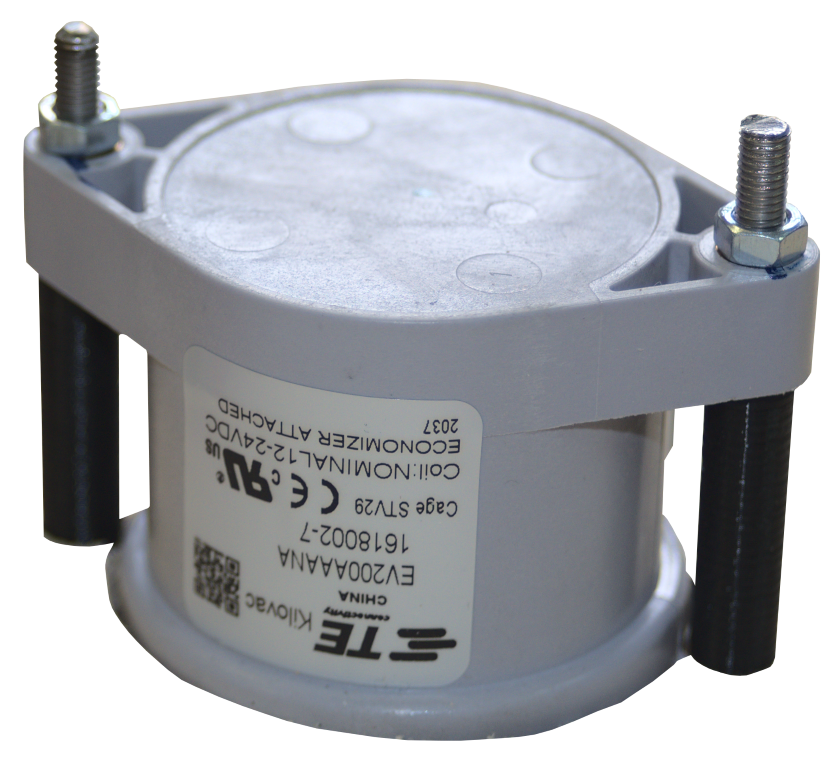
\includegraphics[width=0.45\textwidth]{Fotos/Hauptrelais.png}
    \caption{TE Connectivity EV200 Kfz-Relais}
\end{figure}

\section{Schmelzsicherungen\label{sec:schmelzsicherungen}}
Um im Falle eines Fehlers einen dauerhaften Kurzschluss aller Akkus zu verhindern, wurde sowohl vor als auch nach dem Hauptrelais eine $500\,\mathrm{A}$ Kfz-DC Sicherung verbaut.
\begin{figure}[h]
    \centering
    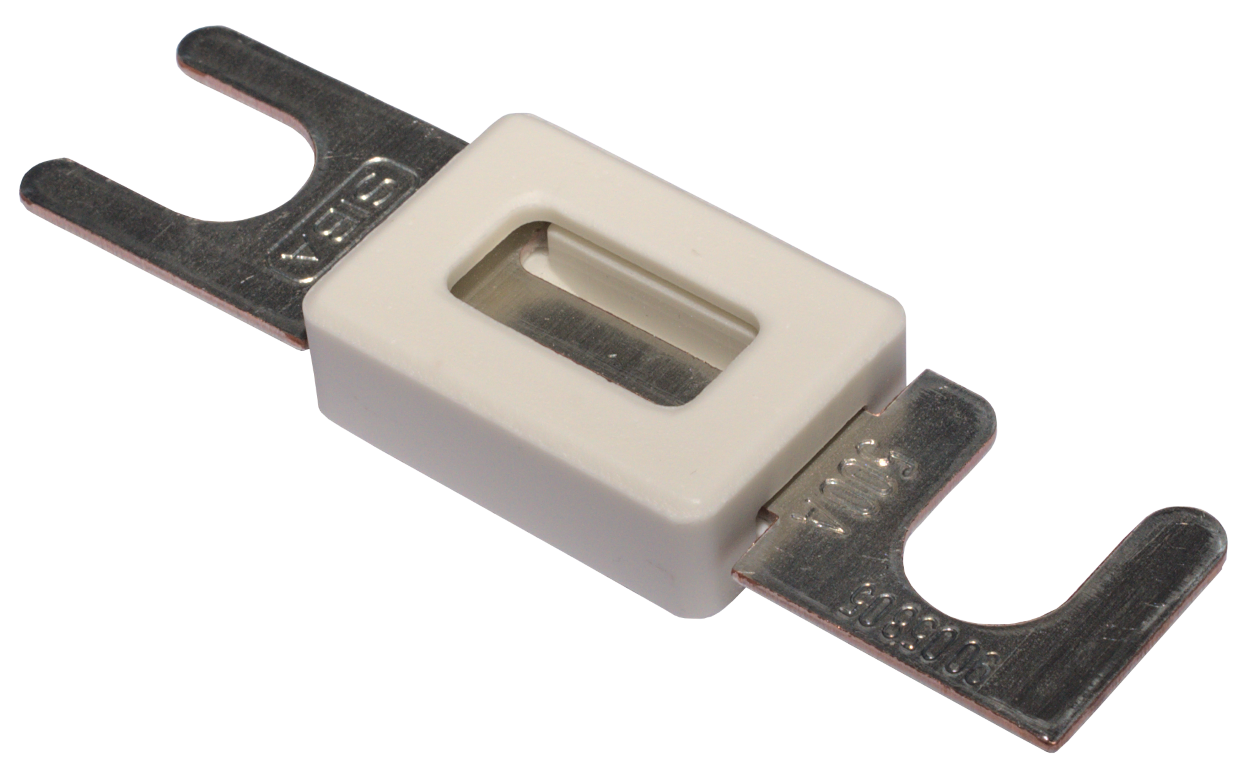
\includegraphics[width=0.55\textwidth]{Fotos/kfz_Sicherung.png}
    \caption{Automotive Kfz Sicherung}
\end{figure}
\newpage

\section{Buck-Converter}
Die Versorgung der Bootelektronik und der Servos übernehmen Buck-Converter, von welchen jeweils einer für ein Servo und einer für die gesamte restliche Elektronik verbaut sind.
\begin{figure}[h]
    \centering
    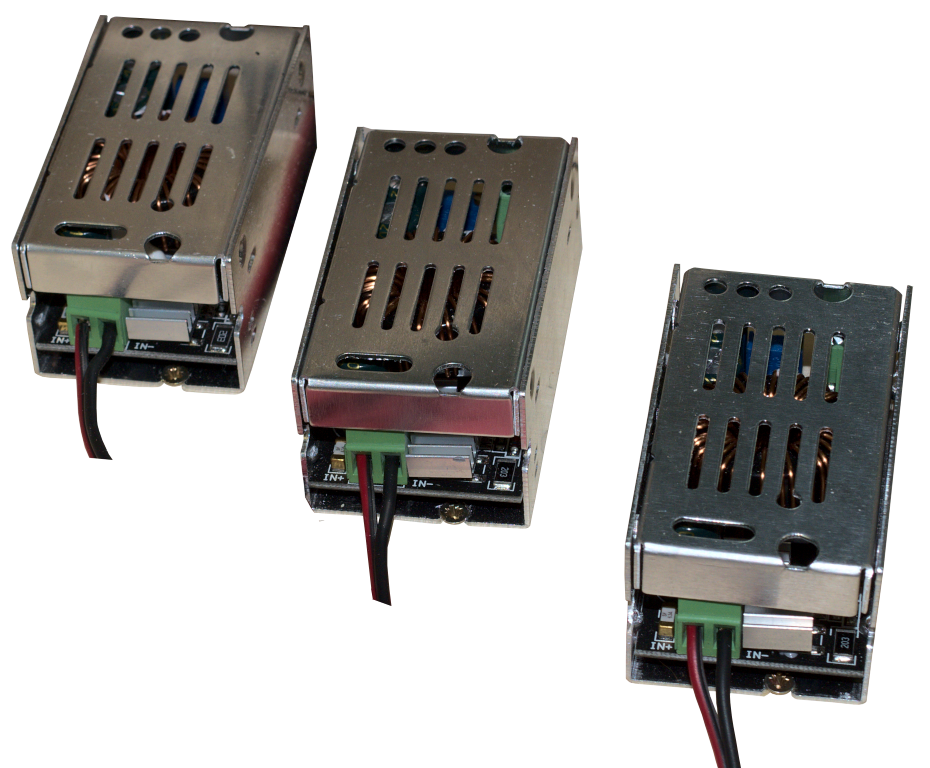
\includegraphics[width=0.8\textwidth]{Fotos/Buck_Converter.png}
    \caption{Buck Converter}
\end{figure}

Wichtig war bei der Auswahl dieser, auf die maximale Eingangsspannung von mindestens $60\,\mathrm{V}$ zu achten. Sehr viele der angebotenen Buck-Converter sind auf $40\,\mathrm{V}$ begrenzt und können daher nicht verwendet werden.
Auch ein Mindeststrom von $6\,\mathrm{A}$ sekundärseitig ist aufgrund des hohen Leistungsbedarfes der Servos vonnöten. 
\newpage

\section{Schaltrelais für Buck-Converter}
Da die negativen Pole beider Akkustränge während des Ladevorganges verbunden werden, müssen die Buck-Converter über eigene Relais abgetrennt werden. 
Um die Schaltströme hierfür möglichst klein zu halten, wird jeder der Converter über ein eigenes Relais geschalten.
\begin{figure}[h]
    \centering
    \includegraphics[width=0.35\textwidth]{Fotos/Relais.png}
    \caption{Relais}
\end{figure}

Hierbei handelt es sich um spezielle DC-Relais, welche für einen Nennstrom von $10\,\mathrm{A}$ ausgelegt sind.
Eine Ansteuerung gemeinsam mit dem Hauptrelais (\ref{sec:hauptrelais}) stellt sicher, dass die Kondensatoren der Buck-Converter vor dem Einschalten über den Leistungswiderstand vorgeladen werden. (siehe \autoref{sec:precharge})

\newpage
\section{Akkus \label{sec:Akkus}}
Nach gründlicher Überlegung, welche Form von Energiespeicher für unser Boot die beste wäre, fiel die Wahl auf die TopFuel LiPo 35C Power-X 7500mAh 7S.
Ursprüngliche Pläne, den Akku selbst aus 18650-Zellen zusammenzubauen, wurden verworfen, da er dadurch bei gleicher speicherbarer Energiemenge deutlich schwerer und auch größer ausgefallen wäre.
\begin{figure}[h]
    \centering
    \includegraphics[width=0.8\textwidth]{Fotos/Akku.png}
    \caption{TopFuel Power-X 7500mAh 7S}
\end{figure}

Auf jeder Seite des Bootes sind, versteckt im hinteren Aufbau, jeweils vier von diesen Akkus verbaut. Mit einer Kapazität von $7500\,\textrm{mAh}$ und einer Nominalspannung von $25.9\,\mathrm{V}$ pro Akku ergibt sich somit eine Gesamtkapazität von zirka $1.55\,\mathrm{kWh}$.

\newpage